\documentclass[xcolor=dvipsnames]{beamer}

\usepackage[utf8]{inputenc}
\usepackage{booktabs}
\usepackage{graphicx}
\usepackage{multimedia}
\usepackage{media9}
\usetheme{PaloAlto}
\usecolortheme[named=RoyalPurple]{structure}
%\setbeamercolor{frametitle}{bg=RoyalPurple}
%\setbeamercolor{sidebar}{bg=RoyalPurple}
%\setbeamercolor{logo}{bg=RoyalPurple!70!black!}

%% TITLE PAGE INFO%%
\title{Using a Genetic Algorithm to Optimize Steel Structures}
\author{Joseph Brown}
\institute{Tarleton State University}
\date{\today}
\graphicspath{ {./figures/} }

\begin{document}
\frame{\titlepage}

\begin{frame}
\begin{center}
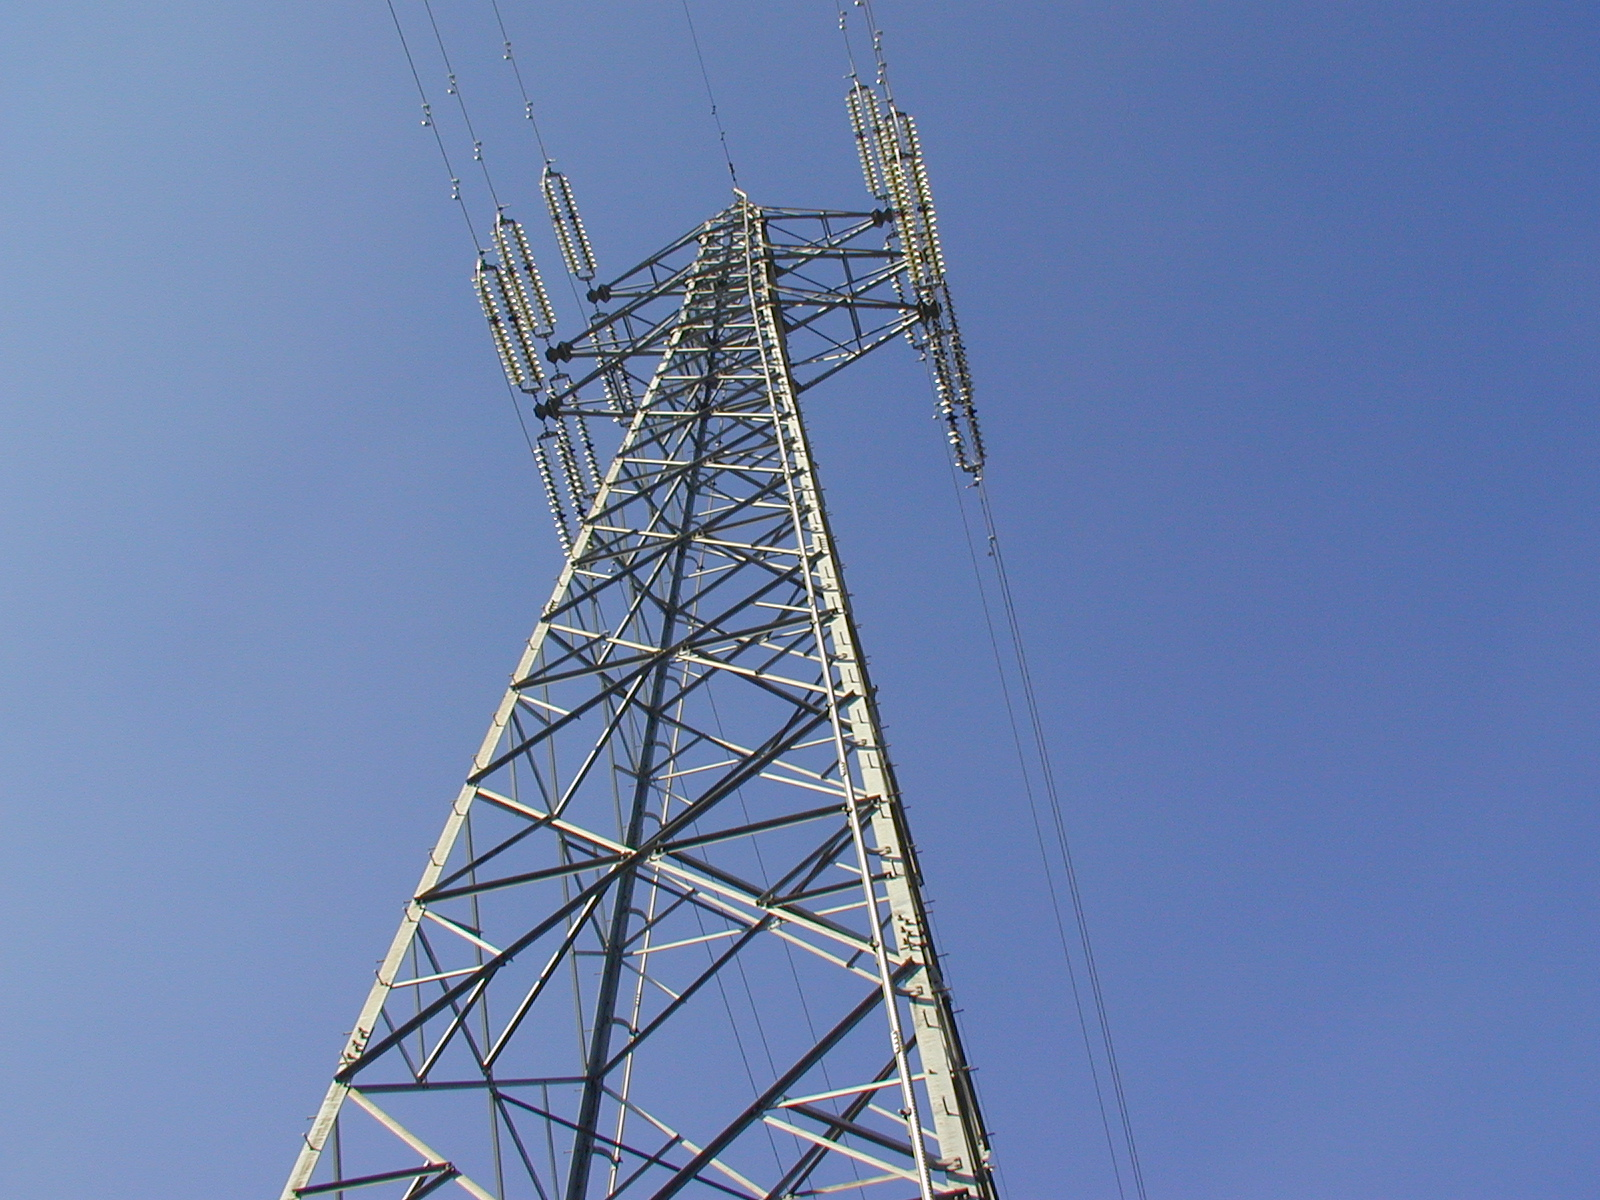
\includegraphics[scale = 0.15]{Steel_tower.jpg}
\end{center}
\end{frame}

\begin{frame}
\begin{center}
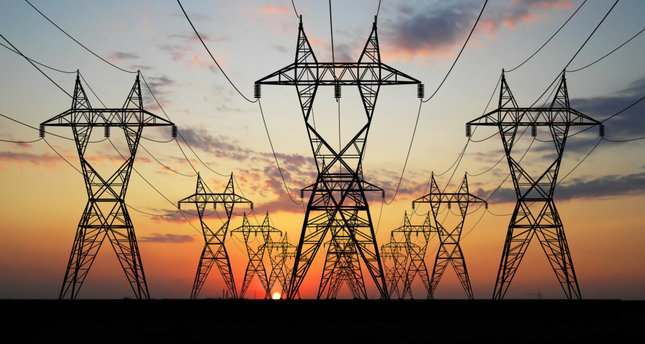
\includegraphics[scale = 0.4]{Steel_tower2.jpg}
\end{center}
\end{frame}

\begin{frame}
\frametitle{Goal \hfill}
\section{Goals/Strategy}	

\begin{itemize}
\item Simulate the physics on a steel structure
\item Determine some metric of ``fitness'' for these structures
\item Systematically breed and cull a population based on this metric.
\end{itemize}
\end{frame}

\begin{frame}
\frametitle{Modeling the Tower}

Steel beams are modeled as springs with a dampening force.  Forces cause the beam to expand or contract, but it will tend to draw its endpoints to a predetermined distance.

Each junction is modeled as an angular spring, pushing or pulling beams at that junction to a predetermined angle.

\end{frame}

\begin{frame}
\begin{center}
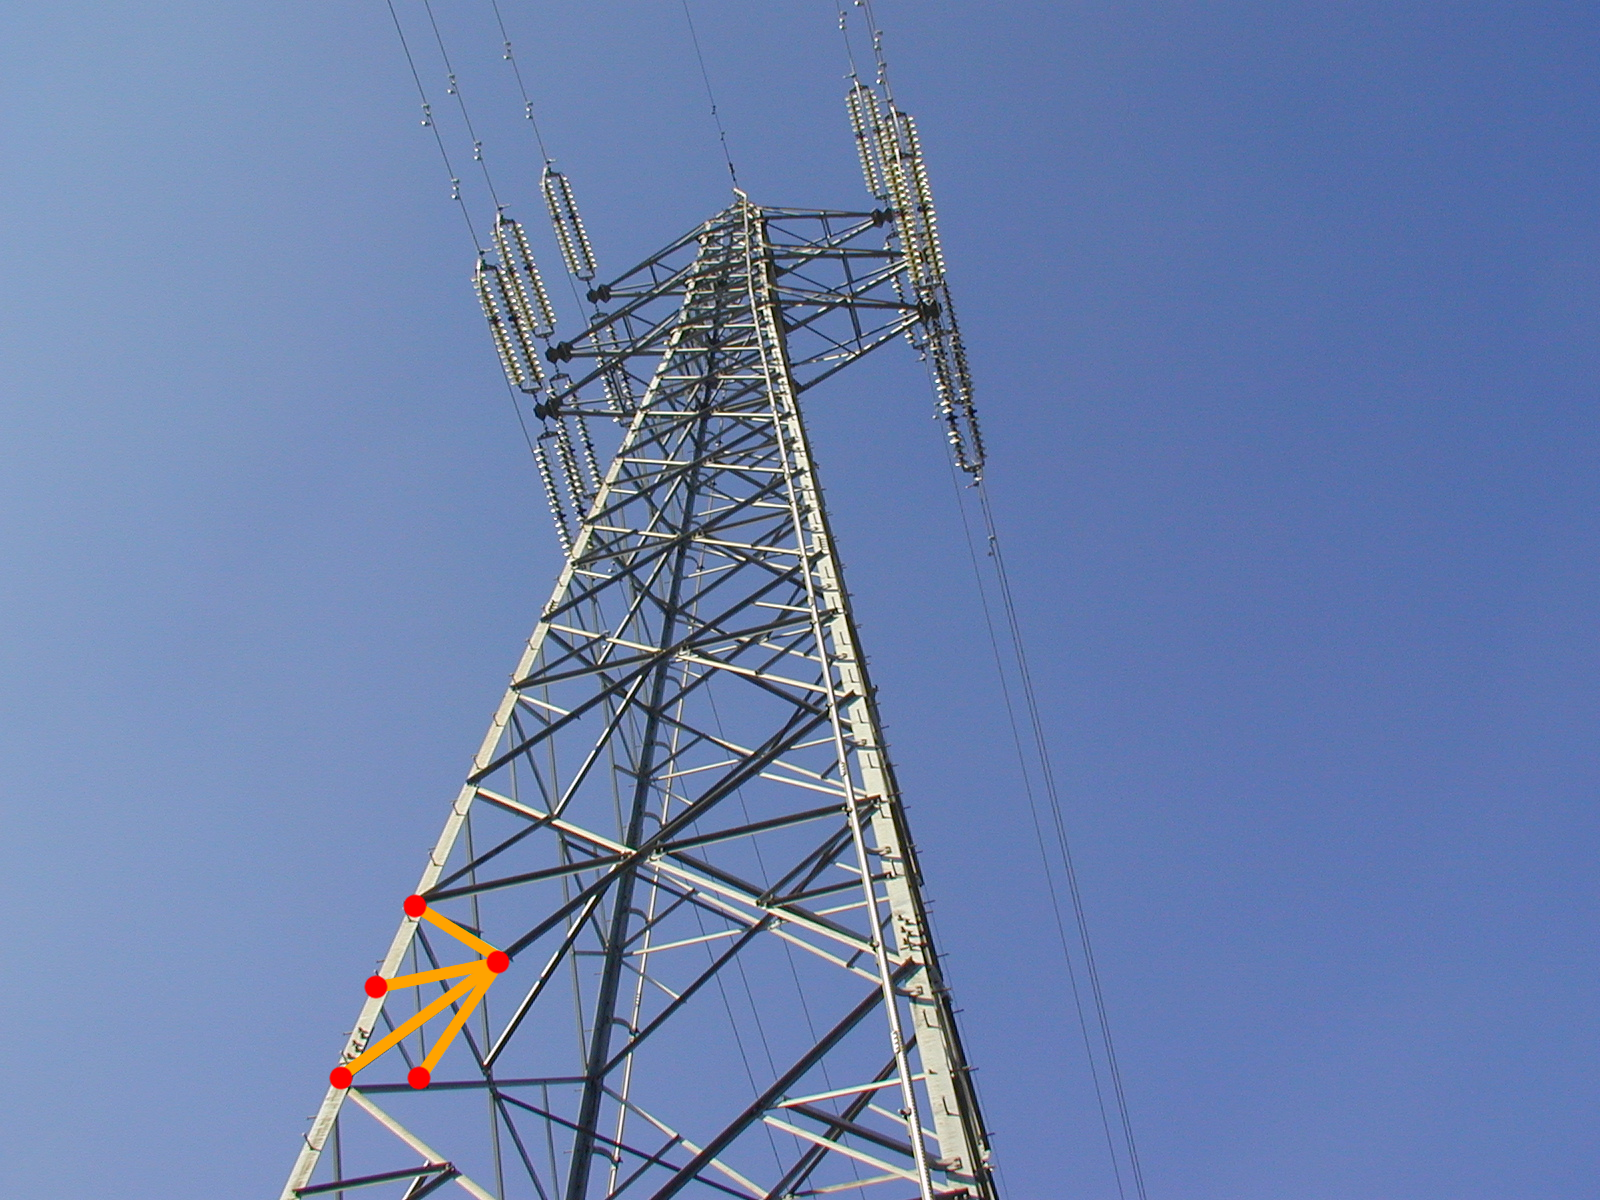
\includegraphics[scale = 0.15]{Steel_tower_model.png}
\end{center}
\end{frame}

\begin{frame}
\section{The Model}	
\frametitle{Genome}

Each tower has a folder containing three files.  One file holds the position of each of its nodes, and whether each node is an anchor point.  A second file holds the information about the beams, including which two nodes are at the ends of the beam, and what the length and spring constant of the beam are.  A third file holds information about angles between beams, and what the angular spring constants are for those junctions.
\begin{center}
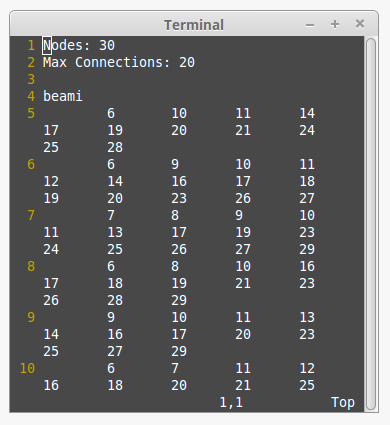
\includegraphics[scale = 0.25]{dongle.png}
\end{center}

\end{frame}

\begin{frame}
\frametitle{Applying that Model to the Genome}

We have a bunch of nodes connected by springs.  We know how the connections are organized, and we know where each of the beams are connected.

By alternately calculating the forces on each node and updating their positions and velocity, we can see how the structure responds to gravity and other external forces.  Using parallel processing on the graphics cards in Dr. Wyatt's lair, I've sped this up a lot.

\end{frame}

\begin{frame}
\begin{center}
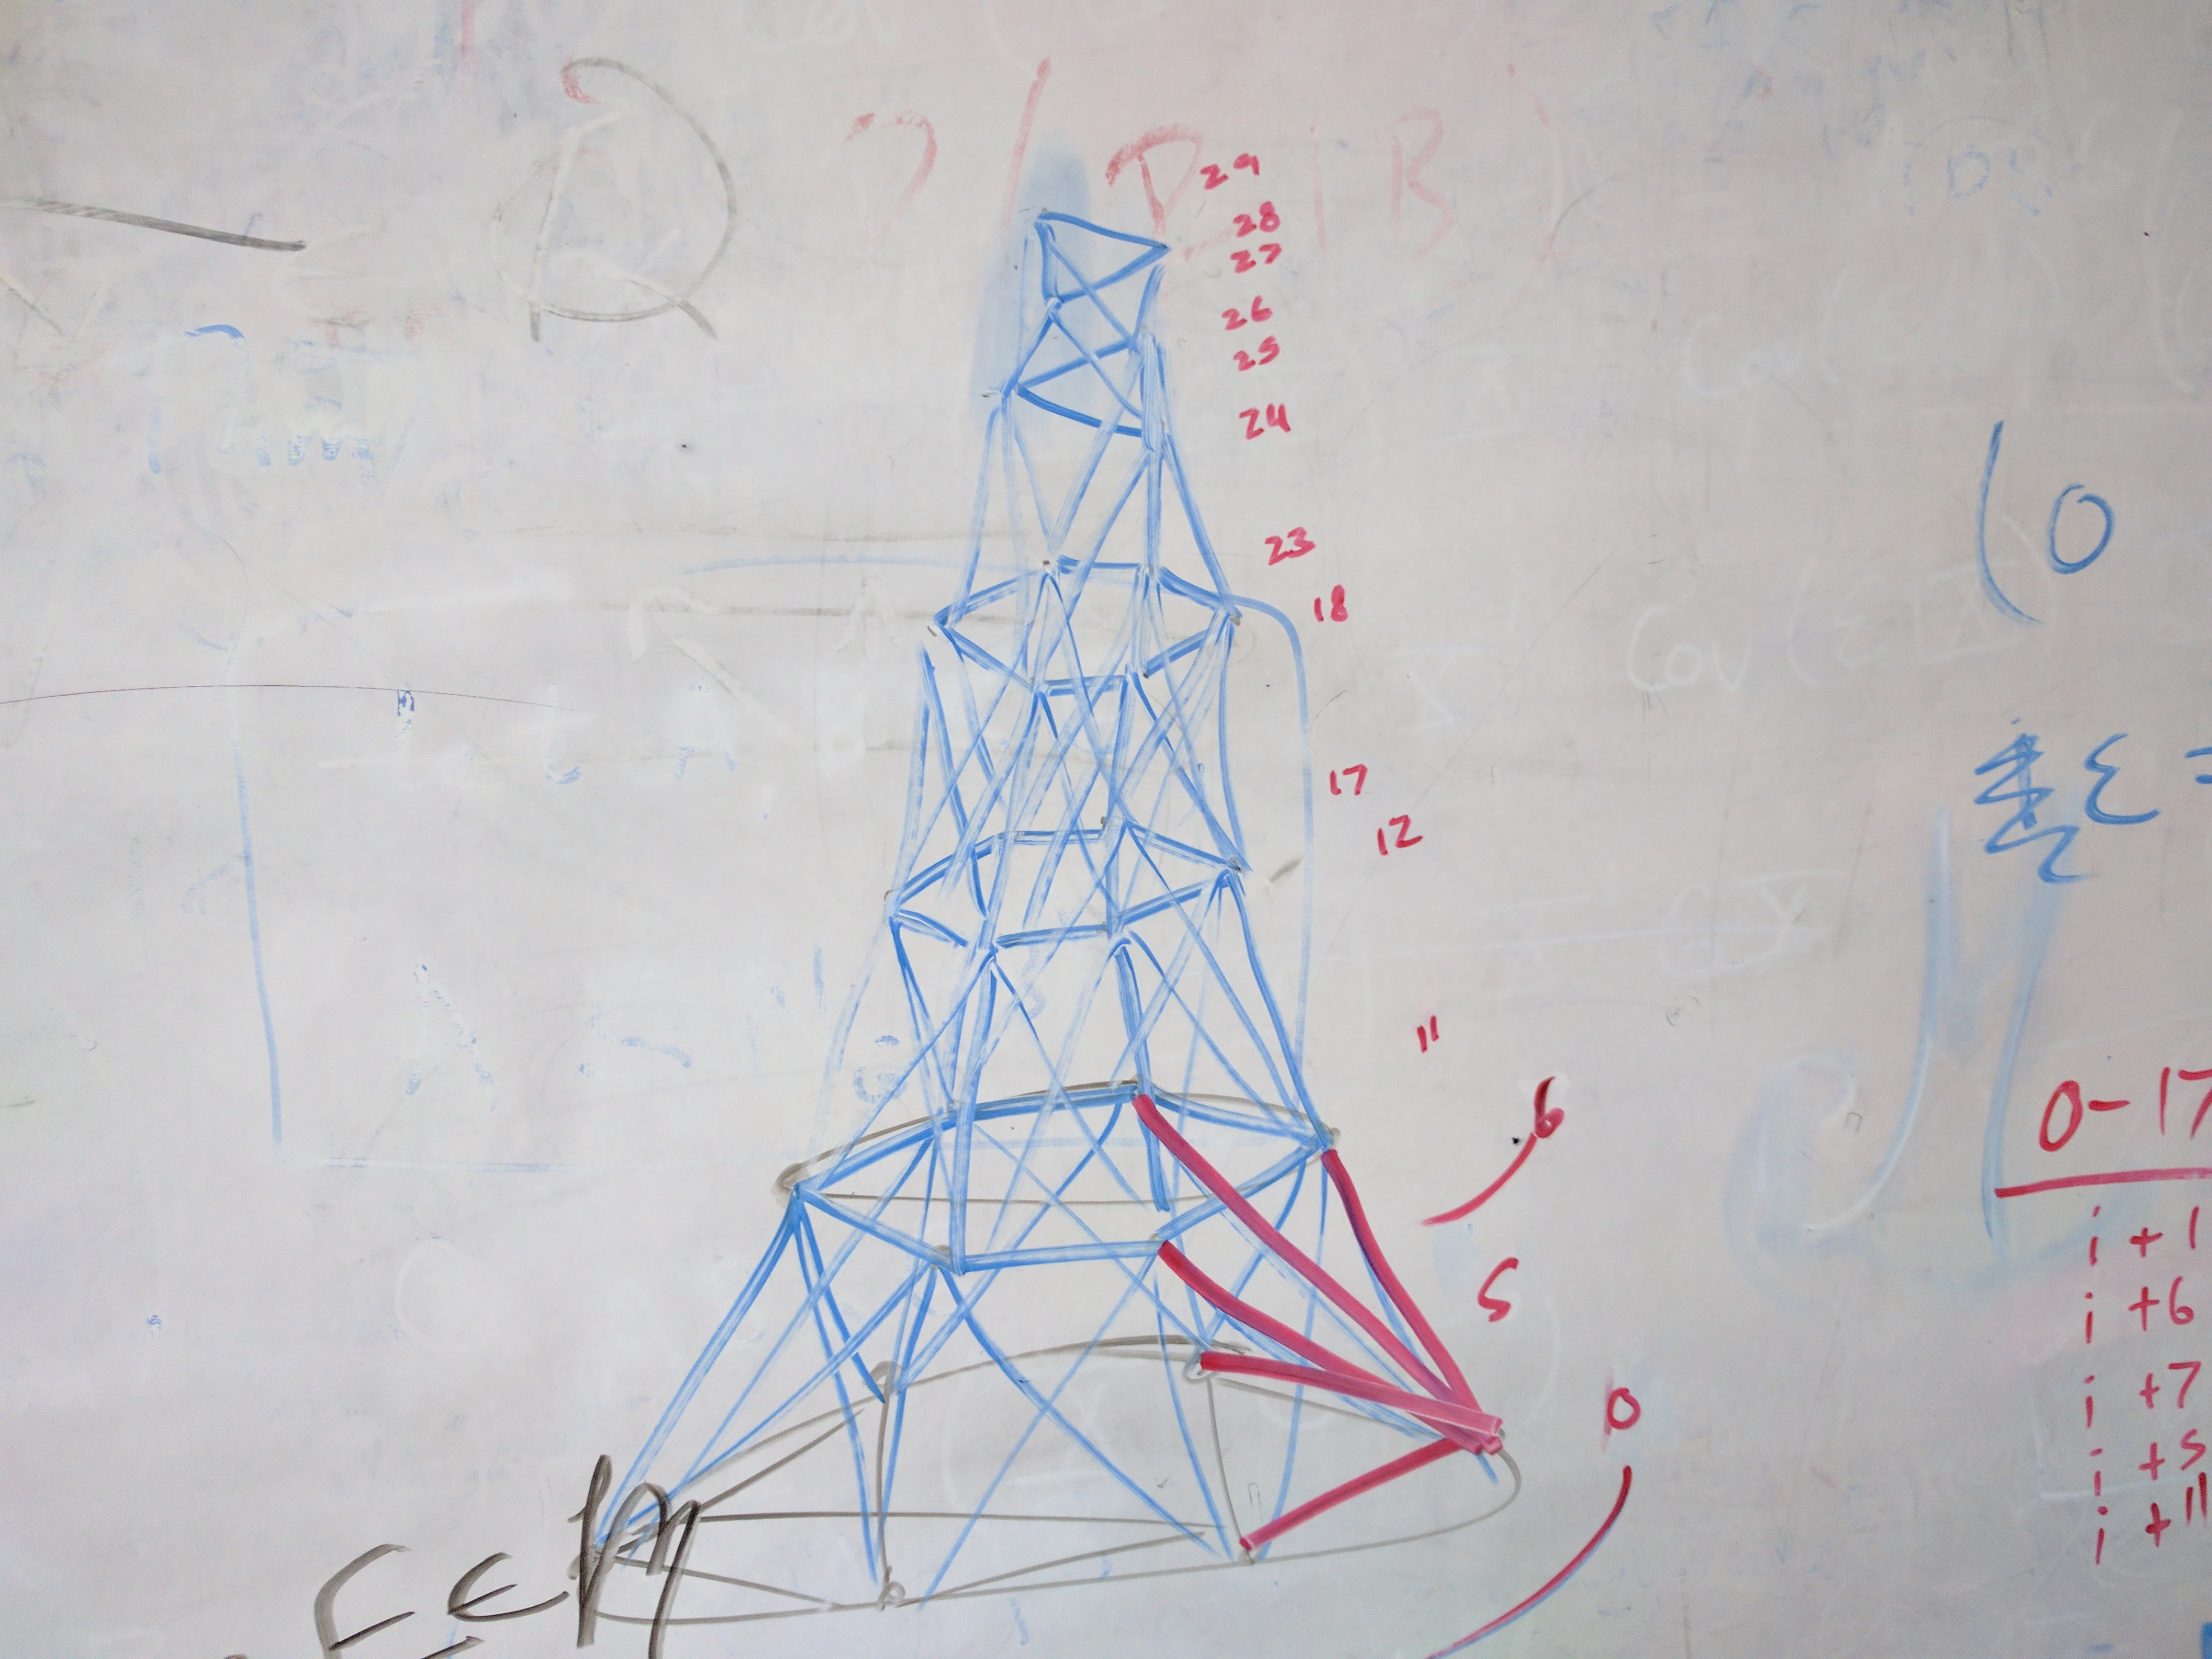
\includegraphics[scale = 0.060]{artTower.jpg}
\end{center}
\end{frame}

\begin{frame}
\section{Evolution}
\frametitle{Evolving}

Population steps
\begin{enumerate}[1]
\item Random Initialization
\item Let structures stabilize and add them to the main population.
\item Remove all structures that have a fitness less than the median.
\item Choose stable structures to be parents based on fitness.
\item Mutate parents to produce children.
\item Let children structures reach a stable state, and add them to the main population.
\item Repeat steps 3-6 until a generation goal is reached.
\end{enumerate}
\end{frame}

\begin{frame}

Random initialization.
(Play random initialization)

\end{frame}

\begin{frame}

Generation 100.
(video)

\end{frame}

\begin{frame}

Generation X.
(video)

\end{frame}

\begin{frame}
\section{This isn't over yet!}
\frametitle{What do my results look like?}
\bigskip

???

\bigskip

?
\end{frame}

\begin{frame}
\frametitle{Room for Improvement}

In actual evolution, entire sequences are spliced together.

Compare to other stochastic processes for building towers.  Metropolis-Hastings?
\end{frame}

\begin{frame}[fragile]

\frametitle{Images}

\tiny
\begin{verbatim}
https://upload.wikimedia.org/wikipedia/commons/d/d0/Steel_tower.jpg

https://iadsb.tmgrup.com.tr/48d616/645/344/0/150/1000/684?
     u=https://idsb.tmgrup.com.tr/2017/03/23/1490217787968.jpg
\end{verbatim}

\end{frame}

\begin{frame}
\frametitle{Thanks!}

\begin{itemize}
\item Dr. Wyatt and his lab
\item Office of Student Research and Creative Activities
\item http://boxcar2d.com
\end{itemize}

\end{frame}

\end{document}